\documentclass[11pt,letterpaper]{article}
\IfFileExists{spanish.ldf}{\usepackage[spanish,es-tabla,es-nodecimaldot]{babel}}{\usepackage{babel}}
\usepackage[utf8]{inputenc}
\usepackage[T1]{fontenc}
\usepackage{lmodern,microtype}
\usepackage[margin=1.8cm,top=1.9cm]{geometry}
\usepackage{amsmath,amssymb}
\usepackage{graphicx,xcolor,booktabs,tabularx,array,enumitem}
\usepackage{titlesec,fancyhdr,float}
\usepackage[hidelinks]{hyperref}
\usepackage{url}

\definecolor{tecnmblue}{RGB}{27,57,106}
\definecolor{accentcolor}{RGB}{229,103,31}
\definecolor{softblue}{RGB}{227,234,246}
\definecolor{softorange}{RGB}{252,236,226}

\titleformat{\section}{\large\bfseries\color{tecnmblue}}{\thesection.}{0.6em}{}
\titleformat{\subsection}{\normalsize\bfseries\color{tecnmblue}}{\thesubsection}{0.6em}{}
\titlespacing*{\section}{0pt}{1.1em}{0.5em}
\setlist{itemsep=2pt,topsep=3pt}
\setlength{\parindent}{0pt}\setlength{\parskip}{4pt}
\renewcommand{\arraystretch}{1.25}
\newcolumntype{Y}{>{\raggedright\arraybackslash}X}
\graphicspath{{img/}}

\pagestyle{fancy}\fancyhf{}
\lhead{\small\color{tecnmblue}Cálculo Vectorial Aplicado · ACF-0904}
\rhead{\small\color{tecnmblue}Proyecto Final U5 · Ejemplo guiado (código DEMO)}
\cfoot{\small\thepage}
\renewcommand{\headrulewidth}{0.4pt}

\newcommand{\paso}[1]{\par\smallskip{\color{accentcolor}\textbf{#1}}\par}
\newcommand{\aviso}[1]{\par\smallskip\colorbox{softorange}{\parbox{\dimexpr\linewidth-2\fboxsep}{\small #1}}\par\smallskip}
\newcommand{\resultado}[1]{\par\colorbox{softblue}{\parbox{\dimexpr\linewidth-2\fboxsep}{#1}}\par}

\begin{document}

\begin{center}
{\LARGE\bfseries\color{tecnmblue} Ejemplo guiado}\\[3pt]
{\large Proyecto Final: validación de la ruta de un AGV}\\[3pt]
{\normalsize Resuelto paso a paso con los datos de práctica (código \texttt{DEMO})}
\end{center}

\aviso{\textbf{Cómo usar este ejemplo.} Aquí se resuelve el proyecto completo con los datos del código \texttt{DEMO}. \textbf{Sus datos son distintos}: copien el método, no los números. Consola: \url{https://thuerta2398.github.io/calculo-vectorial-u5-agv/}}

\section{Paso 1 · Abrir la consola y leer la ficha técnica}
\begin{enumerate}
\item Abran la consola en la computadora o el celular. Al entrar ya carga \texttt{DEMO}; para su planta, escriban su código (\texttt{AGV-XXXX}) y pulsen \emph{Cargar planta}.
\item Copien la \textbf{ficha técnica} en su reporte. Con \texttt{DEMO} queda así:
\end{enumerate}

\begin{center}\small
\begin{tabularx}{0.95\linewidth}{@{}l Y@{}}
\toprule
Ruta & \(\vec r(t)=\langle 4t,\;10\sin(t/2)\rangle,\ t\in[0,4\pi]\) \quad (\(B=10\)) \\
Temperatura & \(T=20+20\,e^{-[(x-13)^2+(y-9)^2]/4^2}\) \quad (\(A=20,\ x_0=13,\ y_0=9,\ \sigma=4\)) \\
Zona de exclusión & disco de radio \(R=5\) m centrado en el horno \((13,9)\) \\
Ventilación & \(\vec F=\langle P,Q\rangle=\langle -0.3\,y+0.002\,x^2,\; 0.02\,xy+1\rangle\) \quad (\(a=0.3,\ b=0.002,\ c=0.02,\ d=1\)) \\
Estabilidad & vía \(w=0.6\) m, altura del centro de gravedad \(h=1.2\) m \\
Almacén & \([32,40]\times[-6,-1]\) m \\ \bottomrule
\end{tabularx}
\end{center}

\aviso{\textbf{Cuidado con los signos.} En la ficha, \(P=-a\,y+b\,x^2\). Si su \(a\) es negativo, el primer término queda positivo: con \(a=-0.4\), \(P=0.4\,y+b\,x^2\).}

\begin{figure}[H]\centering
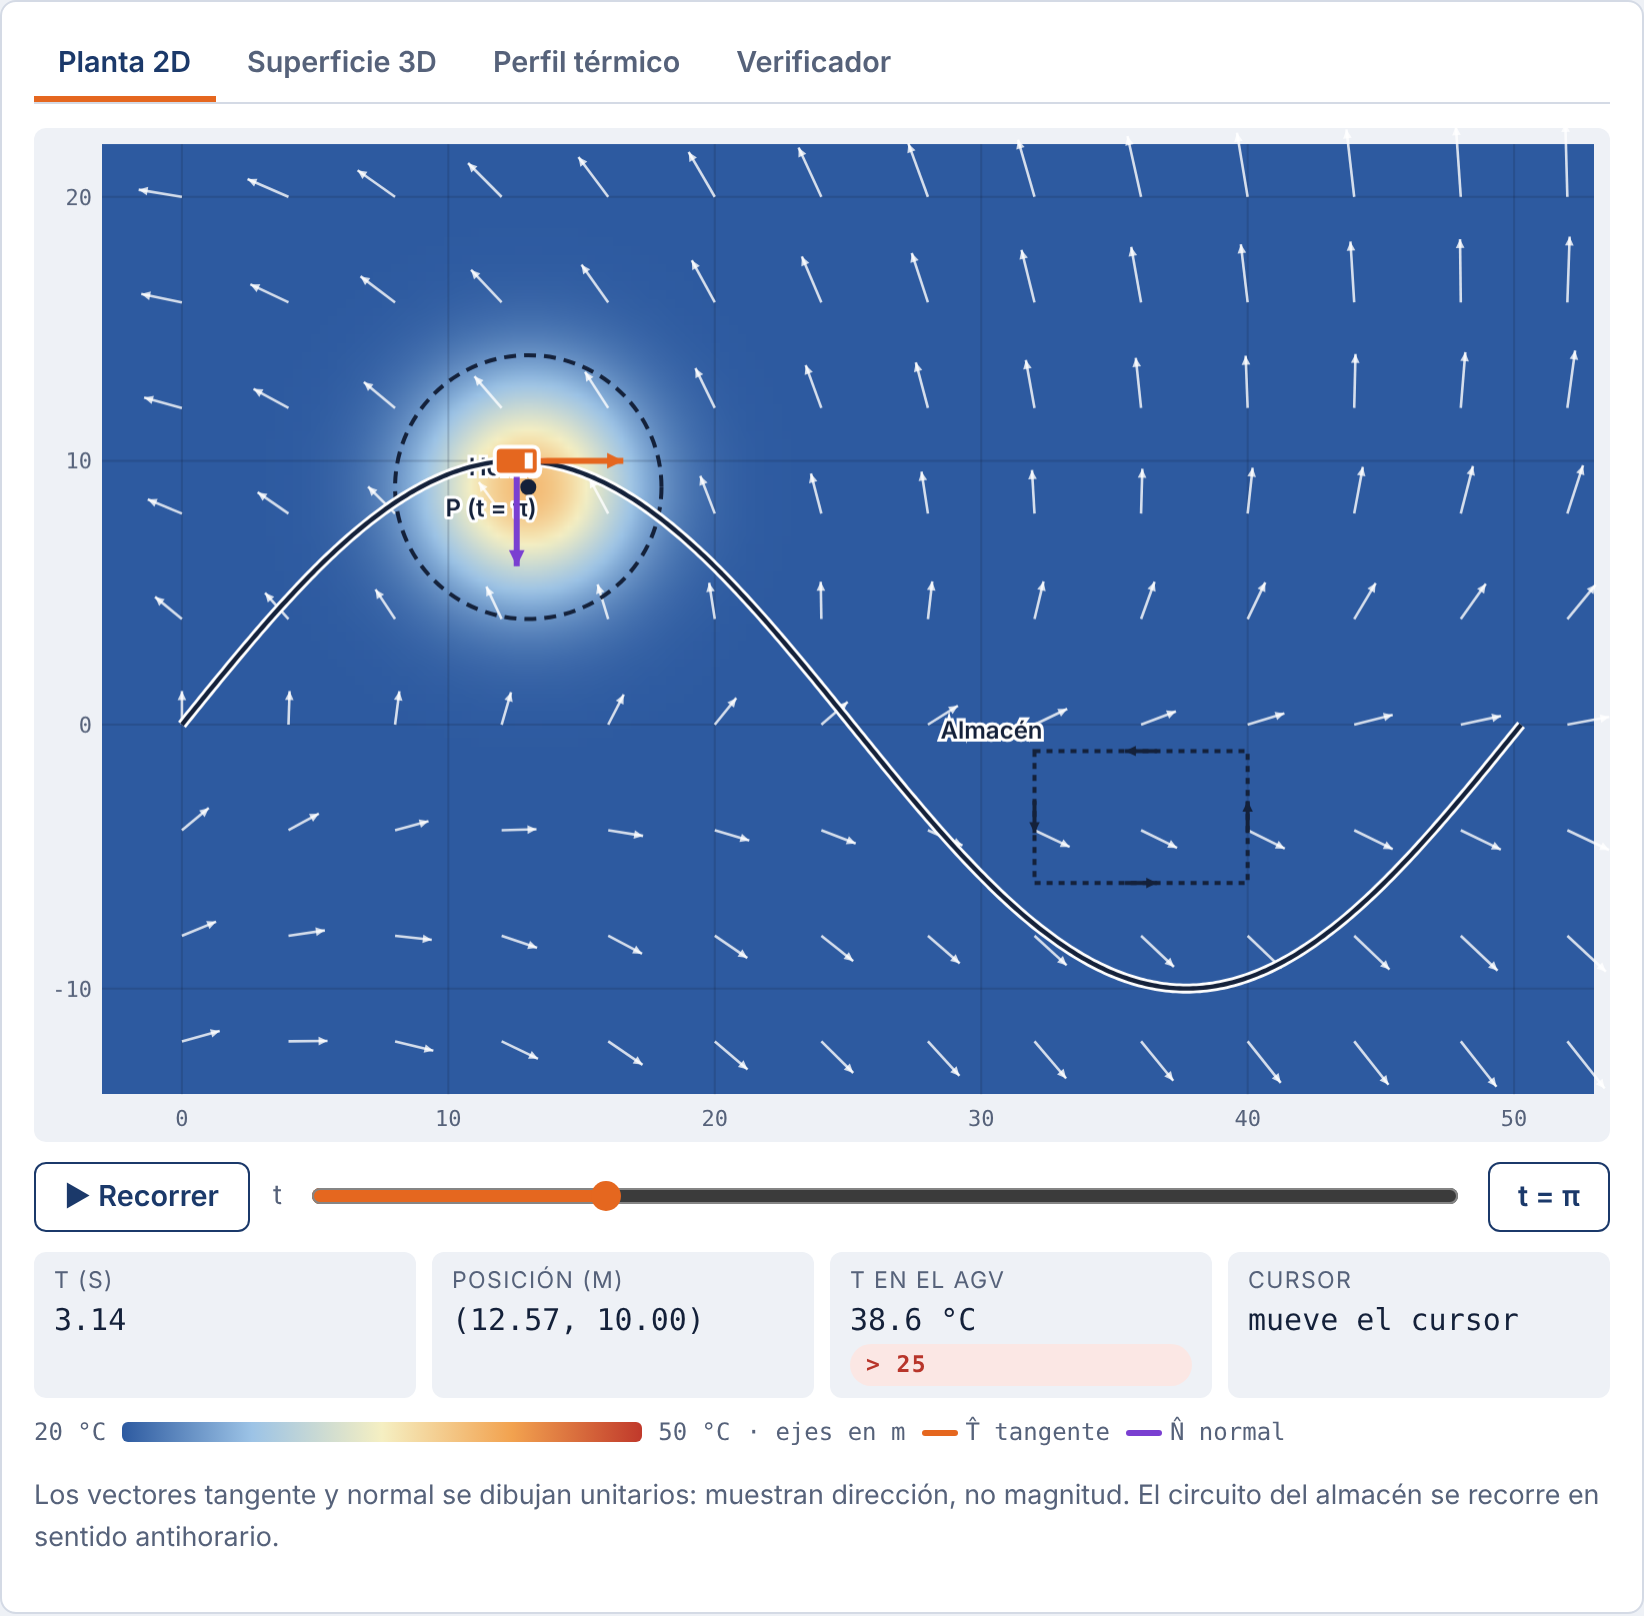
\includegraphics[width=0.92\linewidth]{c2_plano_campo.png}
\caption{Planta 2D con \texttt{DEMO} en \(t=\pi\): mapa de temperatura, ruta, horno con su zona de exclusión, campo \(\vec F\) (flechas blancas), almacén y vectores \(\hat T\) (naranja) y \(\hat N\) (morado). Esta captura sirve como figura del reporte.}
\end{figure}

\paso{Qué observar antes de calcular}
\begin{itemize}
\item Con el deslizador de \(t\), el AGV pasa justo por el disco del horno alrededor de \(t=\pi\): ahí se juntan el riesgo térmico y la curva crítica.
\item El punto crítico es \(P=\vec r(\pi)=(4\pi,\,10\sin(\pi/2))=(4\pi,\,10)\approx(12.57,\,10)\).
\item En \(t=\pi\), \(\hat N\) apunta hacia abajo: la curva gira hacia \(y\) negativas.
\end{itemize}

\section{Paso 2 · Solución por rol}

\subsection*{Ingeniero de Logística: trabajo \(W=\int_C \vec F\cdot d\vec r\), \(t\in[0,2\pi]\)}
\paso{a) Parametrizar}
\(x=4t,\quad y=10\sin(t/2),\quad dx=4\,dt,\quad dy=5\cos(t/2)\,dt.\)

\paso{b) Sustituir en \(P\) y \(Q\)}
\[P=-0.3(10\sin\tfrac t2)+0.002(4t)^2=-3\sin\tfrac t2+0.032\,t^2,\qquad
Q=0.02(4t)(10\sin\tfrac t2)+1=0.8\,t\sin\tfrac t2+1.\]

\paso{c) Armar el integrando \(P\,dx+Q\,dy\)}
\[P\,dx=\big(-12\sin\tfrac t2+0.128\,t^2\big)dt,\qquad
Q\,dy=\big(4t\sin\tfrac t2\cos\tfrac t2+5\cos\tfrac t2\big)dt=\big(2t\sin t+5\cos\tfrac t2\big)dt,\]
porque \(2\sin\tfrac t2\cos\tfrac t2=\sin t\).

\paso{d) Integrar término a término}
\begin{align*}
\int_0^{2\pi}-12\sin\tfrac t2\,dt &= \Big[24\cos\tfrac t2\Big]_0^{2\pi}=24(-1-1)=-48\\
\int_0^{2\pi}0.128\,t^2\,dt &= 0.128\cdot\frac{(2\pi)^3}{3}=\frac{1.024\,\pi^3}{3}\approx 10.5835\\
\int_0^{2\pi}2t\sin t\,dt &= 2\Big[-t\cos t+\sin t\Big]_0^{2\pi}=2(-2\pi)=-4\pi\approx-12.5664\\
\int_0^{2\pi}5\cos\tfrac t2\,dt &= \Big[10\sin\tfrac t2\Big]_0^{2\pi}=0
\end{align*}
La tercera integral se resuelve por partes con \(u=t\), \(dv=\sin t\,dt\).
\resultado{\(W=-48+10.5835-12.5664\approx \mathbf{-49.98\ J}\). El trabajo es negativo: en el primer tramo la ventilación \textbf{se opone} al avance del AGV.}

\subsection*{Ingeniero de Dinámica: divergencia, rotacional y aceleración normal}
\paso{a) Derivadas parciales}
\(\dfrac{\partial P}{\partial x}=0.004\,x,\quad \dfrac{\partial P}{\partial y}=-0.3,\quad \dfrac{\partial Q}{\partial x}=0.02\,y,\quad \dfrac{\partial Q}{\partial y}=0.02\,x.\)

\paso{b) Divergencia y rotacional en \(P=(4\pi,10)\)}
\begin{align*}
\operatorname{div}\vec F&=0.004x+0.02x=0.024x &&\Rightarrow\; 0.024(4\pi)\approx \mathbf{0.30}\\
(\operatorname{rot}\vec F)\cdot\hat k&=0.02y-(-0.3)=0.02y+0.3 &&\Rightarrow\; 0.02(10)+0.3=\mathbf{0.50}
\end{align*}
Interpretación: \(\operatorname{div}>0\), así que en \(P\) el aire sale del punto (\textbf{fuente}); \(\operatorname{rot}>0\), así que tiende a girar en sentido \textbf{antihorario}.

\paso{c) Aceleración normal en \(t=\pi\)}
\(\vec r\,'(t)=\langle 4,\,5\cos\tfrac t2\rangle,\quad \vec r\,''(t)=\langle 0,\,-2.5\sin\tfrac t2\rangle\). En \(t=\pi\): \(\vec r\,'=\langle 4,0\rangle\) (rapidez 4 m/s) y \(\vec r\,''=\langle 0,-2.5\rangle\).
\[a_N=\frac{|x'y''-y'x''|}{\|\vec r\,'\|}=\frac{|4(-2.5)-0\cdot 0|}{4}=\mathbf{2.50\ m/s^2},\qquad
a_{\text{lím}}=\frac{g\,w}{2h}=\frac{9.81(0.6)}{2(1.2)}\approx 2.45\ \text{m/s}^2.\]
\resultado{\(a_N=2.50>a_{\text{lím}}=2.45\): con \texttt{DEMO}, el AGV \textbf{vuelca} en la curva crítica, aunque por un margen pequeño (2\,\%).}

\subsection*{Ingeniero Térmico: integral doble en polares}
\paso{a) Plantear en polares centradas en el horno}
Con \(x=13+r\cos\theta,\ y=9+r\sin\theta\), se cumple \((x-13)^2+(y-9)^2=r^2\) y \(dA=r\,dr\,d\theta\):
\[\iint_D (T-20)\,dA=\int_0^{2\pi}\!\!\int_0^{5}20\,e^{-r^2/16}\,r\,dr\,d\theta .\]
\paso{b) Resolver con \(u=r^2/16\), \(du=\tfrac{r}{8}dr\)}
\[\int_0^5 e^{-r^2/16}\,r\,dr=8\int_0^{25/16}e^{-u}\,du=8\big(1-e^{-25/16}\big)\approx 8(1-0.20961)=6.3231.\]
\[\iint_D (T-20)\,dA=2\pi\cdot 20\cdot 6.3231\approx \mathbf{794.59\ °C\cdot m^2}\qquad\big(=\pi A\sigma^2(1-e^{-R^2/\sigma^2})\big).\]
\paso{c) Temperatura promedio}
\resultado{\(\bar T=20+\dfrac{794.59}{\pi(5)^2}=20+\dfrac{794.59}{78.54}\approx \mathbf{30.12\ °C}>25\ °C\). La zona del horno debe declararse \textbf{de exclusión}.}

\subsection*{Gerente de Calidad: teorema de Green en el almacén \([32,40]\times[-6,-1]\)}
\paso{a) Lado derecho de Green (integral doble)}
\[\iint_R\Big(\frac{\partial Q}{\partial x}-\frac{\partial P}{\partial y}\Big)dA=\int_{32}^{40}\!\int_{-6}^{-1}(0.02y+0.3)\,dy\,dx
=8\Big[0.01y^2+0.3y\Big]_{-6}^{-1}=8\big[(-0.29)-(-1.44)\big]=\mathbf{9.20}.\]
\paso{b) Lado izquierdo (integral de línea, cuatro lados en sentido antihorario)}
\begin{center}\small
\begin{tabular}{@{}llll@{}}\toprule
Lado & Recorrido & Integral & Valor\\\midrule
\(C_1\) abajo & \(y=-6\), \(x:32\to40\), \(dy=0\) & \(\int_{32}^{40}(1.8+0.002x^2)\,dx\) & \(35.2213\)\\
\(C_2\) derecha & \(x=40\), \(y:-6\to-1\), \(dx=0\) & \(\int_{-6}^{-1}(0.8y+1)\,dy\) & \(-9.0000\)\\
\(C_3\) arriba & \(y=-1\), \(x:40\to32\), \(dy=0\) & \(\int_{40}^{32}(0.3+0.002x^2)\,dx\) & \(-23.2213\)\\
\(C_4\) izquierda & \(x=32\), \(y:-1\to-6\), \(dx=0\) & \(\int_{-1}^{-6}(0.64y+1)\,dy\) & \(6.2000\)\\\midrule
& & \textbf{Suma} & \(\mathbf{9.2000}\)\\\bottomrule
\end{tabular}\end{center}
\resultado{Los dos métodos dan \(\oint_C\vec F\cdot d\vec r=\mathbf{9.20\ J}\): se comprueba el teorema de Green. Una circulación positiva indica \textbf{recirculación antihoraria del aire} en el almacén, que puede mantener polvo en suspensión sobre los componentes.}

\section{Paso 3 · Verificar los resultados}
\paso{En la consola (pestaña Verificador)}
Capturen cada resultado con \textbf{punto decimal}, sin unidades. Si usan coma, la consola lo indica y ese intento no cuenta:
\begin{center}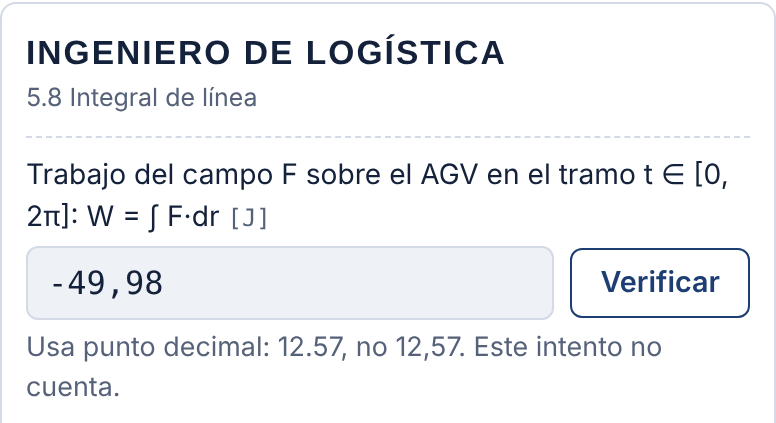
\includegraphics[width=0.42\linewidth]{c4_coma.png}\end{center}
Con los 7 resultados correctos aparece el folio. Con \texttt{DEMO} solo se muestra ``Práctica completa''; con su código aparece un folio del tipo \texttt{AGV-XXXX-1A2B3C4}, que va en la portada.
\begin{figure}[H]\centering
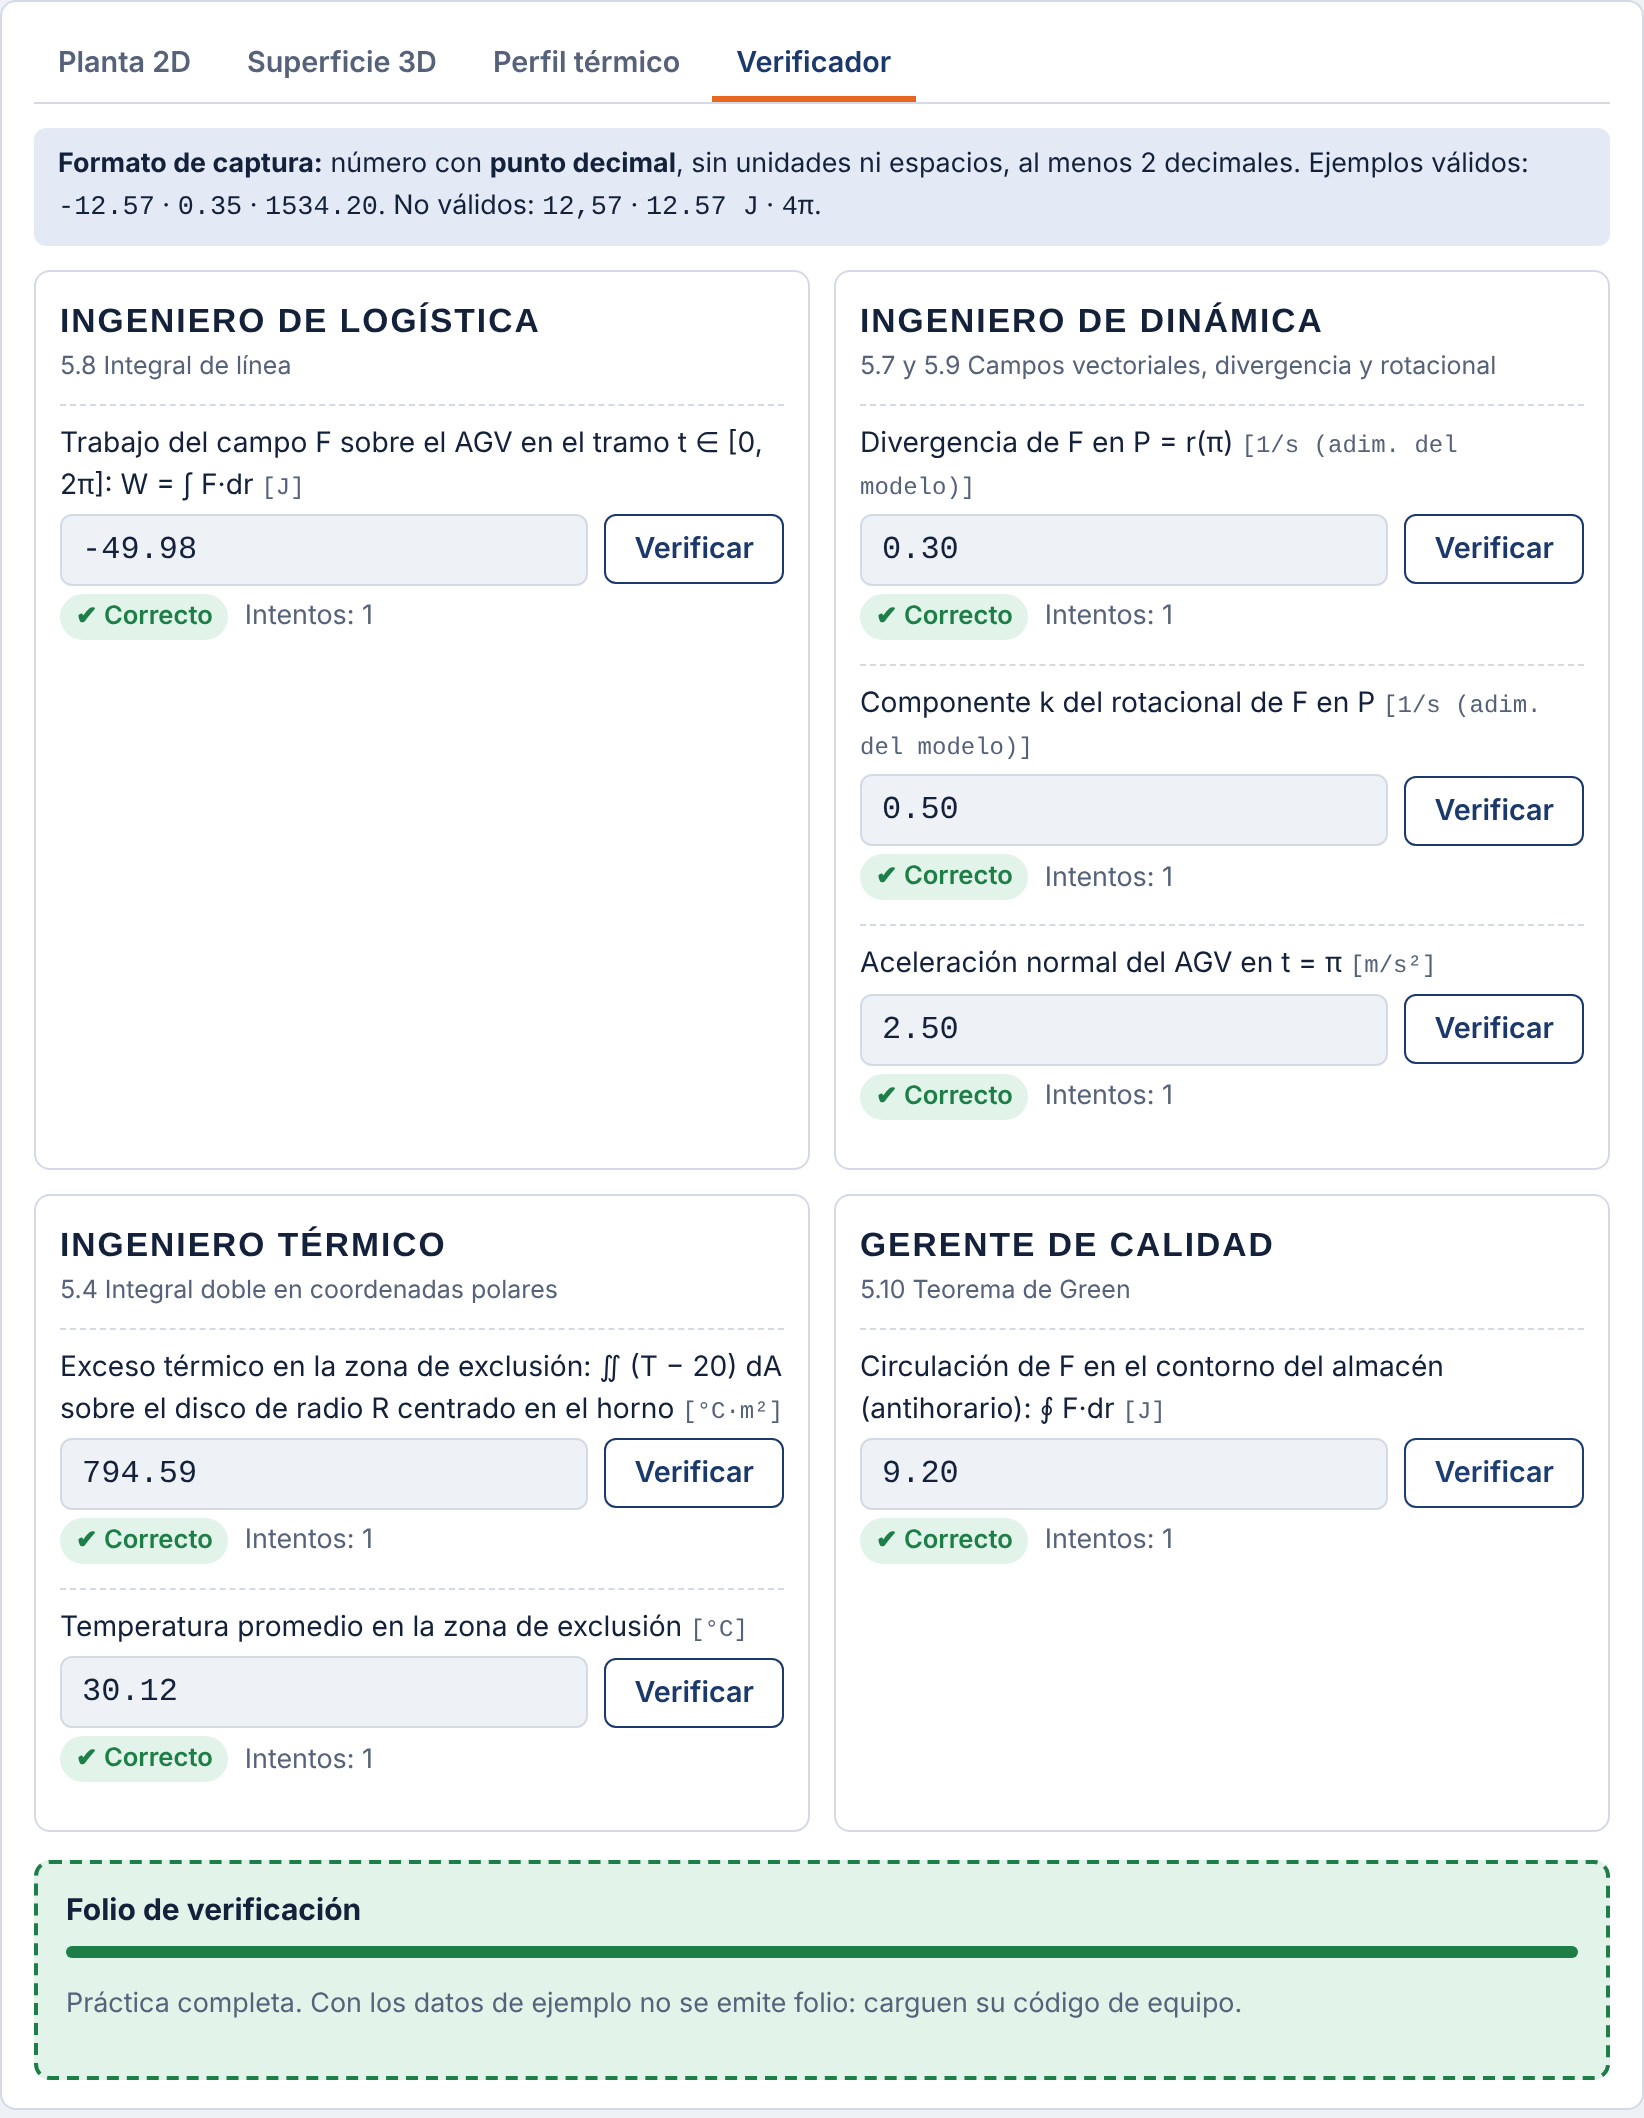
\includegraphics[width=0.62\linewidth]{c5_verificador.png}
\caption{Verificador con los 7 resultados de \texttt{DEMO} correctos.}
\end{figure}

\paso{En Wolfram Alpha (opcional, para comprobar un paso)}
Escriban en \url{https://www.wolframalpha.com} instrucciones como estas, cambiando los números por los suyos:
\begin{itemize}\small
\item \texttt{integrate (-12 sin(t/2) + 0.128 t\^{}2 + 2 t sin(t) + 5 cos(t/2)) dt from t=0 to 2pi}
\item \texttt{integrate 20*exp(-r\^{}2/16)*r dr dtheta, r=0..5, theta=0..2pi}
\item \texttt{integrate (0.02 y + 0.3) dy dx, y=-6..-1, x=32..40}
\end{itemize}
Wolfram comprueba el número, pero en el reporte debe aparecer \textbf{su procedimiento}.

\section{Paso 4 · Leer el perfil térmico}
\begin{figure}[H]\centering
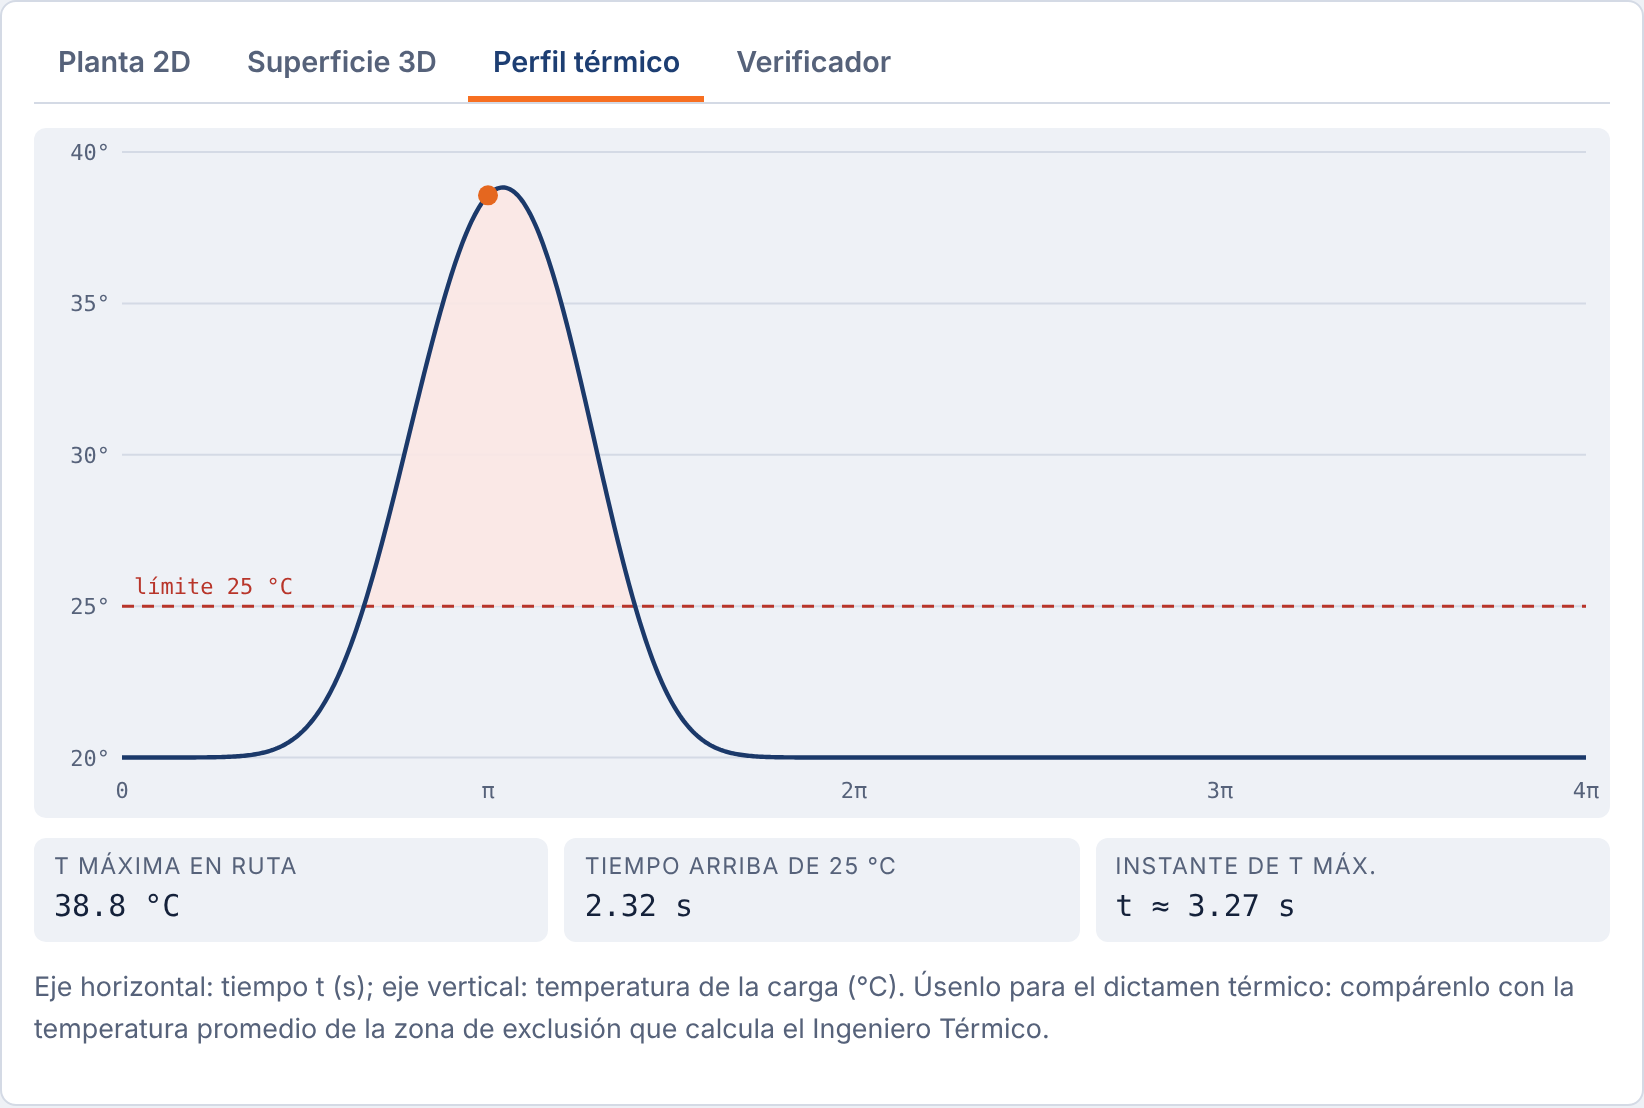
\includegraphics[width=0.85\linewidth]{c3_perfil.png}
\caption{Perfil térmico de \texttt{DEMO}: la zona sombreada es el tiempo en que la carga supera 25\,°C.}
\end{figure}
Con \texttt{DEMO}, la carga alcanza \(T_{\max}\approx 38.8\) °C cerca de \(t\approx 3.27\) s y pasa unos \textbf{2.33 s} arriba de 25\,°C, entre \(t\approx 2.08\) y \(4.40\) s.

\section{Paso 5 · Redactar el dictamen (ejemplo)}
\resultado{\small\textbf{Dictamen de ingeniería (código DEMO).}
\textbf{Seguridad cinética:} en \(t=\pi\) la aceleración normal es \(a_N=2.50\) m/s\(^2\), mayor que el límite de vuelco \(a_{\text{lím}}=2.45\) m/s\(^2\). El AGV vuelca en la curva crítica; se recomienda reducir la amplitud de la curva o la velocidad en ese tramo.
\textbf{Riesgo térmico:} la temperatura promedio de la zona del horno es 30.12\,°C, superior al límite de 25\,°C, y el perfil muestra que la carga pasa 2.33 s arriba de ese límite, con un máximo de 38.8\,°C. La ruta cruza la zona de exclusión.
\textbf{Ventilación:} el trabajo en el primer tramo es \(W=-49.98\) J, así que el aire frena al AGV. En \(P\), \(\operatorname{div}\vec F=0.30>0\) (fuente) y \(\operatorname{rot}\vec F=0.50>0\) (giro antihorario). En el almacén, la circulación de 9.20 J, comprobada con Green, indica recirculación de aire.
\textbf{Decisión: ruta rechazada} en su forma actual. Se aprobaría con condiciones si se desvía la ruta fuera del disco del horno y se suaviza la curva crítica.}

Fíjense en que cada afirmación del dictamen \textbf{usa un número calculado} y termina en una consecuencia para la planta.

\section{Paso 6 · Armar la entrega}
\subsection*{Portada (ejemplo)}
\begin{center}\small
\begin{tabularx}{0.9\linewidth}{@{}l Y@{}}\toprule
Código de equipo & \texttt{AGV-XXXX} \\
Folio de verificación & \texttt{AGV-XXXX-1A2B3C4} (el que da su consola) \\
Integrantes y rol & Nombre 1: Logística · Nombre 2: Dinámica · Nombre 3: Térmico · Nombre 4: Calidad \\
Video & \url{https://drive.google.com/file/d/...} \\ \bottomrule
\end{tabularx}\end{center}

\subsection*{El reporte en PDF (máximo 4 cuartillas, sin contar la portada)}
\begin{itemize}
\item \textbf{Word:} \emph{Insertar \(\rightarrow\) Ecuación} para las fórmulas; al terminar, \emph{Archivo \(\rightarrow\) Guardar como \(\rightarrow\) PDF}.
\item \textbf{Google Docs:} \emph{Insertar \(\rightarrow\) Ecuación}; al terminar, \emph{Archivo \(\rightarrow\) Descargar \(\rightarrow\) Documento PDF}.
\item \textbf{Procedimiento a mano:} es válido si se lee bien. Escaneen con la app de Google Drive (botón \emph{+} \(\rightarrow\) \emph{Escanear}) o con Microsoft Lens e inserten las imágenes en el documento.
\item \textbf{Capturas de la consola:} en Windows, \texttt{Win + Shift + S}; en Mac, \texttt{Cmd + Shift + 4}. Pónganles pie de figura.
\item Para no pasarse de 4 cuartillas: una sección por rol (½ a ¾ de cuartilla cada una), dos o tres figuras y el dictamen al final.
\end{itemize}

\subsection*{El video (4:30 a 5:30 min, todos a cuadro, con rotación de roles)}
\begin{enumerate}
\item \textbf{Grabar:} hagan una videollamada en Zoom o Teams con las cuatro cámaras encendidas, compartan la consola en pantalla y graben la reunión. Otra opción es grabar la pantalla: en Windows, \texttt{Win + Alt + R} (Xbox Game Bar); en Mac, \texttt{Cmd + Shift + 5}.
\item \textbf{Guion sugerido}, alrededor de 1 min por persona: Logística explica Dinámica, Dinámica explica Térmico, Térmico explica Calidad y Calidad explica Logística. Cierren con el dictamen en 30 s.
\item \textbf{Subir a Drive:} \emph{drive.google.com \(\rightarrow\) Nuevo \(\rightarrow\) Subir archivo}.
\item \textbf{Compartir:} clic derecho sobre el video \(\rightarrow\) \emph{Compartir} \(\rightarrow\) en \emph{Acceso general} elijan \textbf{``Cualquier persona con el enlace''}, con rol \textbf{Lector} \(\rightarrow\) \emph{Copiar vínculo}.
\item \textbf{Probar:} abran el vínculo en una ventana de incógnito (\texttt{Ctrl + Shift + N} en Chrome). Si pide iniciar sesión, el permiso está mal y el video valdría 0.
\end{enumerate}

\section{Errores frecuentes}
\begin{center}\small
\begin{tabularx}{\linewidth}{@{}>{\raggedright\arraybackslash}p{5.2cm} Y@{}}\toprule
\textbf{Error} & \textbf{Cómo evitarlo}\\\midrule
Calculadora en grados & Las integrales y \(\sin t\) usan \textbf{radianes}. \\
Olvidar \(dx\) o \(dy\) en la integral de línea & \(dx=x'(t)\,dt\) y \(dy=y'(t)\,dt\): sin ellos el resultado sale mal. \\
Olvidar el factor \(r\) en polares & \(dA=r\,dr\,d\theta\), no \(dr\,d\theta\). \\
Recorrer el almacén en sentido horario & Green exige sentido \textbf{antihorario}; en sentido horario cambia el signo. \\
Usar el punto equivocado & \(P=\vec r(\pi)=(4\pi,\,B)\), no \((\pi,B)\). \\
Coma decimal o unidades en el verificador & \texttt{-49.98}, no \texttt{-49,98} ni \texttt{-49.98 J}. \\
Leer en el video & Ensayen una vez; usen la consola como apoyo visual, no un guion. \\ \bottomrule
\end{tabularx}\end{center}

\end{document}
